\documentclass[journal,12pt,twocolumn]{IEEEtran}
\usepackage{amsthm}
\usepackage{gensymb}
\usepackage{setspace}
\singlespacing
\usepackage[cmex10]{amsmath}
\usepackage{bm}

\usepackage{cases}
\usepackage{mathrsfs}
\usepackage{cite}
\usepackage{stfloats}
\usepackage{mathtools}
\usepackage[breaklinks=true]{hyperref}
\usepackage{graphicx}
\usepackage{subfig}
\usepackage{txfonts}
\usepackage{longtable}
\usepackage{multirow}
\usepackage{tfrupee}
\usepackage{enumitem}
\usepackage{tikz}
\usetikzlibrary{automata, positioning}
\usepackage{steinmetz}
\usepackage{verbatim}
\usepackage{circuitikz}
\usepackage{tkz-euclide}





\usetikzlibrary{calc,math}
\usepackage{listings}
    \usepackage{color}                                            %%
    \usepackage{array}                                            %%
    \usepackage{longtable}                                        %%
    \usepackage{calc}                                             %%
    \usepackage{multirow}                                         %%
    \usepackage{hhline}                                           %%
    \usepackage{ifthen}                                           %%
    \usepackage{lscape}     
\usepackage{multicol}
\usepackage{chngcntr}

\DeclareMathOperator*{\Res}{Res}

\renewcommand\thesection{\arabic{section}}
\renewcommand\thesubsection{\thesection.\arabic{subsection}}
\renewcommand\thesubsubsection{\thesubsection.\arabic{subsubsection}}

\renewcommand \thesectiondis{\arabic{section}}
\renewcommand\thesubsectiondis{\thesectiondis.\arabic{subsection}}
\renewcommand\thesubsubsectiondis{\thesubsectiondis.\arabic{subsubsection}}


\hyphenation{op-tical net-works semi-conduc-tor}
\def\inputGnumericTable{}                                 %%

\lstset{
%language=C,
frame=single, 
breaklines=true,
columns=fullflexible
}
\begin{document}

\newcommand{\BEQA}{\begin{eqnarray}}
\newcommand{\EEQA}{\end{eqnarray}}
\newcommand{\define}{\stackrel{\triangle}{=}}
\bibliographystyle{IEEEtran}
\raggedbottom
\setlength{\parindent}{0pt}
\providecommand{\mbf}{\mathbf}
\providecommand{\pr}[1]{\ensuremath{\Pr\left(#1\right)}}
\providecommand{\qfunc}[1]{\ensuremath{Q\left(#1\right)}}
\providecommand{\sbrak}[1]{\ensuremath{{}\left[#1\right]}}
\providecommand{\lsbrak}[1]{\ensuremath{{}\left[#1\right.}}
\providecommand{\rsbrak}[1]{\ensuremath{{}\left.#1\right]}}
\providecommand{\brak}[1]{\ensuremath{\left(#1\right)}}
\providecommand{\lbrak}[1]{\ensuremath{\left(#1\right.}}
\providecommand{\rbrak}[1]{\ensuremath{\left.#1\right)}}
\providecommand{\cbrak}[1]{\ensuremath{\left\{#1\right\}}}
\providecommand{\lcbrak}[1]{\ensuremath{\left\{#1\right.}}
\providecommand{\rcbrak}[1]{\ensuremath{\left.#1\right\}}}
\theoremstyle{remark}
\newtheorem{rem}{Remark}
\newcommand{\sgn}{\mathop{\mathrm{sgn}}}
\providecommand{\abs}[1]{\vert#1\vert}
\providecommand{\res}[1]{\Res\displaylimits_{#1}} 
\providecommand{\norm}[1]{\lVert#1\rVert}
%\providecommand{\norm}[1]{\lVert#1\rVert}
\providecommand{\mtx}[1]{\mathbf{#1}}
\providecommand{\mean}[1]{E[ #1 ]}
\providecommand{\fourier}{\overset{\mathcal{F}}{ \rightleftharpoons}}
%\providecommand{\hilbert}{\overset{\mathcal{H}}{ \rightleftharpoons}}
\providecommand{\system}{\overset{\mathcal{H}}{ \longleftrightarrow}}
	%\newcommand{\solution}[2]{\textbf{Solution:}{#1}}
\newcommand{\solution}{\noindent \textbf{Solution: }}
\newcommand{\cosec}{\,\text{cosec}\,}
\providecommand{\dec}[2]{\ensuremath{\overset{#1}{\underset{#2}{\gtrless}}}}
\newcommand{\myvec}[1]{\ensuremath{\begin{pmatrix}#1\end{pmatrix}}}
\newcommand{\mydet}[1]{\ensuremath{\begin{vmatrix}#1\end{vmatrix}}}
\numberwithin{equation}{subsection}
\makeatletter
\@addtoreset{figure}{problem}
\makeatother
\let\StandardTheFigure\thefigure
\let\vec\mathbf
\renewcommand{\thefigure}{\theproblem}
\def\putbox#1#2#3{\makebox[0in][l]{\makebox[#1][l]{}\raisebox{\baselineskip}[0in][0in]{\raisebox{#2}[0in][0in]{#3}}}}
     \def\rightbox#1{\makebox[0in][r]{#1}}
     \def\centbox#1{\makebox[0in]{#1}}
     \def\topbox#1{\raisebox{-\baselineskip}[0in][0in]{#1}}
     \def\midbox#1{\raisebox{-0.5\baselineskip}[0in][0in]{#1}}
\vspace{3cm}
\title{Assignment7}%number
\author{CS20Btech11035 -NYALAPOGULA MANASWINI}
\maketitle
\newpage
\bigskip

\renewcommand{\thefigure}{\theenumi}
\renewcommand{\thetable}{\theenumi}
Download python code from 
\begin{lstlisting}
https://github.com/N-Manaswini23/assignment7/tree/main/python%20codes
\end{lstlisting}
%
Download latex code from 
\begin{lstlisting}
https://github.com/N-Manaswini23/assignment7/blob/main/assignment7.tex
\end{lstlisting}
%

\section*{CSIR UGC NET EXAM(Dec 2016) Q-49}
There are two boxes. Box-$1$ contains $2$ red balls and $4$ green balls. Box-$2$ contains $4$ red balls and $2$ green balls. A box is selected at random and a ball is chosen randomly from the selected box. If the ball turns out to be red, what is the probability that Box-$1$ had been selected?
\section*{SOLUTION}
Box-$1$ has $2$ red balls and $4$ green balls.\\
Box-$2$ has $4$ red balls and $2$ green balls.\\
Let $B \in \{1,2\} $ represent a random variable where $1$ represents selecting box-$1$ and $2$ represents selecting box-$2$.

\begin{table}[h!]
\resizebox{9cm}{!}
{ 
\begin{tabular}{|c|c|c|}
\hline
Event & definition & value\\
\hline
$ \pr{B=1} $ & Probability of selecting  & $\frac{1}{2}$\\
&Box-$1$ & \\
\hline
$ \pr{B=2} $ & Probability of selecting & $\frac{1}{2}$ \\
& Box-$2$& \\
\hline
$\pr{R=1|B=1}$ & Probability of drawing &  $\frac{1}{3}$   \\
&  red ball from Box-$1$ &\\
\hline
$\pr{G=1|B=1}$ & Probability of drawing &  $\frac{2}{3}$   \\
&  green ball from Box-$1$ &\\
\hline
$\pr{R=1|B=2}$ & Probability of drawing &  $\frac{2}{3}$   \\
&  red ball from Box-$2$ &\\
\hline
$\pr{G=1|B=2}$ & Probability of drawing &  $\frac{1}{3}$   \\
&  green ball from Box-$2$ &\\
\hline
\end{tabular}
}
\caption{Table 1} 
\label{tab:1}
\end{table}


From Baye's theorem
\begin{align}
\pr{R=1}&=\pr{R=1|B=1} \times \pr{B=1} \notag \\
 & +\pr{R=1|B=2} \times \pr{B=2}  \label{1}
 \end{align}
Substiting values from table \eqref{tab:1} in \eqref{1}
\begin{align}
\pr{R=1} &=\frac{1}{2} \label{2} \\
\pr{(R=1)(B=1)}&=\pr{R=1|B=1}\notag \\
&  \times \pr{B=1} \\ 
&= \frac{1}{6}  \label{3}
\end{align}
We need to find $\pr{B=1|R=1}$ \\
\begin{align}
\pr{B=1|R=1} &= \frac{\pr{(R=1 ) (B=1)}}{\pr{R=1}} \\
&=\frac{1}{3}
\end{align}

 $\therefore$ The desired probability that box-$1$ is selected $= \frac{1}{3}$ \\
 

 
\begin{figure}[htb!]
\begin{center}
\includegraphics[width=0.5\textwidth]{assignment7theory.png}
\end{center}
\end{figure}

\begin{figure}[htb!]
\begin{center}
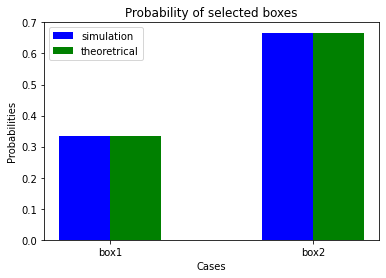
\includegraphics[width=0.5\textwidth]{assignment7sim.png}
\end{center}
\end{figure}

\end{document}